\documentclass{article}
\usepackage{graphicx}
\usepackage{booktabs}
\usepackage{amsmath}
\usepackage{hyperref}
\usepackage{siunitx}
\usepackage{amsfonts}
\usepackage[hyperpageref]{backref}
\usepackage[alf]{abntex2cite}
\usepackage[margin=0.75in]{geometry}
\begin{document}
\title{BIOS 611 Final Project}
\author{Yixiang Qu \\ e-mail: yqu@unc.edu}
\date{October 28, 2021}
\maketitle

\section{Introduction}
With progress on both the theoretical and the computational fronts, the use of spline modelling has become an established tool in statistical regression analysis. In particular, splines are regularly used for building explanatory models in clinical research. Indeed, many new methodological developments in modern biostatistics make use of splines to model smooth functions of interest. However, when it comes to very complicated model structure, traditional splines methods may not work well and may not help to make use of all the information. In my first year of my PhD, I made a deep learning tool for better interpolate microbiome data. In order to compare its performance with traditional spline methods, I made this project. It will use Rshiny to show the difference of the interpolation results of my deep learning method and the B-spline method.

\section{The complicated data structure of microbiome time series data}

The time series data two dimensions originally. However, since there are multiply observations of microbiome species at one time point, the dataset has three dimensions, called a multivariate time series dataset.

Consider a $N$-subject time series dataset with $V$-dimensional covariates. We can use $j \in \{1,2,\ldots,N \}$ to denote the $j$-th subject. For the $j$-th subject with $L_j$ samples, we use $\mathbf{T_j} = (t_{j,1}, t_{j,2}, \ldots, t_{j,L_j})$ to denote the observation time points. And for the $i$-th ($i \in\{1,2, \ldots, L_j\}$) time point, the observation values $\mathbf{y_{j,i}}$ will be a $V$-dimensional vector. Therefore, for the $j$-th subject, we can denote the observation values as $\mathbf{Y_j}\in \mathbb{R}^{L_{j}\times V}$. And if there are missing values in the $j$-th subject, we can use mask matrix $\mathbf{M_j}\in\{0,1\}^{L_{j}\times V}$ to indicate the missing information, where 0 indicated that the information is missing at the specific time point for the certain subject.

\begin{table}[h!]
  \centering
  \caption{A example data format of multivariate microbiome time series dataset}
    \begin{tabular}{c|c|c|c|c|c|c|c|c|c}
    ID    & Time  & Value\_1 & Value\_2 & {$\ldots$} & Value\_V & Mask\_1 & Mask\_2 & {$\ldots$} & Mask\_V \\ \midrule
    {1} & $t_{1,1}$ & $y_{1,1,1}$ & $y_{1,1,2}$ &       & $y_{1,1,V}$ & $m_{1,1,1}$ & $m_{1,1,2}$ &       & $m_{1,1,V}$ \\ \hline
    {1} & $t_{1,2}$ & $y_{1,2,1}$ & $y_{1,2,2}$ &       & $y_{1,2,V}$ & $m_{1,2,1}$ & $m_{1,2,2}$ &       & $m_{1,2,V}$ \\ \hline
    {1} & $t_{1,3}$ & $y_{1,3,1}$ & $y_{1,3,2}$ &       & $y_{1,3,V}$ & $m_{1,3,1}$ & $m_{1,3,2}$ &       & $m_{1,3,V}$ \\ \hline
    {2} & $t_{2,1}$ & $y_{2,1,1}$ & $y_{2,1,2}$ &       & $y_{2,1,V}$ & $m_{2,1,1}$ & $m_{2,1,2}$ &       & $m_{2,1,V}$ \\ \hline
    {2} & $t_{2,2}$ & $y_{2,2,1}$ & $y_{2,2,2}$ &       & $y_{2,2,V}$ & $m_{2,2,1}$ & $m_{2,2,2}$ &       & $m_{2,2,V}$ \\ \hline
    $\ldots$ &       &       &       &       &       &       &       &       &  \\ \hline
    j     & $t_{j,1}$ & $y_{j,1,1}$ & $y_{j,1,2}$ &       & $y_{j,1,V}$ & $m_{j,1,1}$ & $m_{j,1,2}$ &       & $m_{j,1,V}$ \\ \hline
    j     & $t_{j,2}$ & $y_{j,2,1}$ & $y_{j,2,2}$ &       & $y_{j,2,V}$ & $m_{j,2,1}$ & $m_{j,2,2}$ &       & $m_{j,2,V}$ \\ \hline
    $\ldots$ &       &       &       &       &       &       &       &       &  \\ \hline
    j     & $t_{j,L_j}$ & $y_{j,L_j,1}$ & $y_{j,L_j,2}$ &       & $y_{j,L_j,V}$ & $m_{j,L_j,1}$ & $m_{j,L_j,2}$ &       & $m_{j,L_j,V}$ \\ \hline
    $\ldots$ &       &       &       &       &       &       &       &       &  \\ \hline
    N     & $t_{N,1}$ & $y_{N,1,1}$ & $y_{N,1,2}$ &       & $y_{N,1,V}$ & $m_{N,1,1}$ & $m_{N,1,2}$ &       & $m_{N,1,V}$ \\ \hline
    N     & $t_{N,2}$ & $y_{N,2,1}$ & $y_{N,2,2}$ &       & $y_{N,2,V}$ & $m_{N,2,1}$ & $m_{N,2,2}$ &       & $m_{N,2,V}$ \\ \hline
    N     & $t_{N,3}$ & $y_{N,3,1}$ & $y_{N,3,2}$ &       & $y_{N,3,V}$ & $m_{N,3,1}$ & $m_{N,3,2}$ &       & $m_{N,3,V}$ \\ 
    \end{tabular}
\label{input_format}
\end{table}

\section{Interpolation results of different spline methods}

\subsection{Deep learning interpolation}\label{sec3}

The model to interpolate the time series data is related to my paper, which is under preperation, so I apologize that I cannot write too much details in the report. A concise diagram is shown as Fig. \ref{diagram}.

\begin{figure}[h]
    \centering
    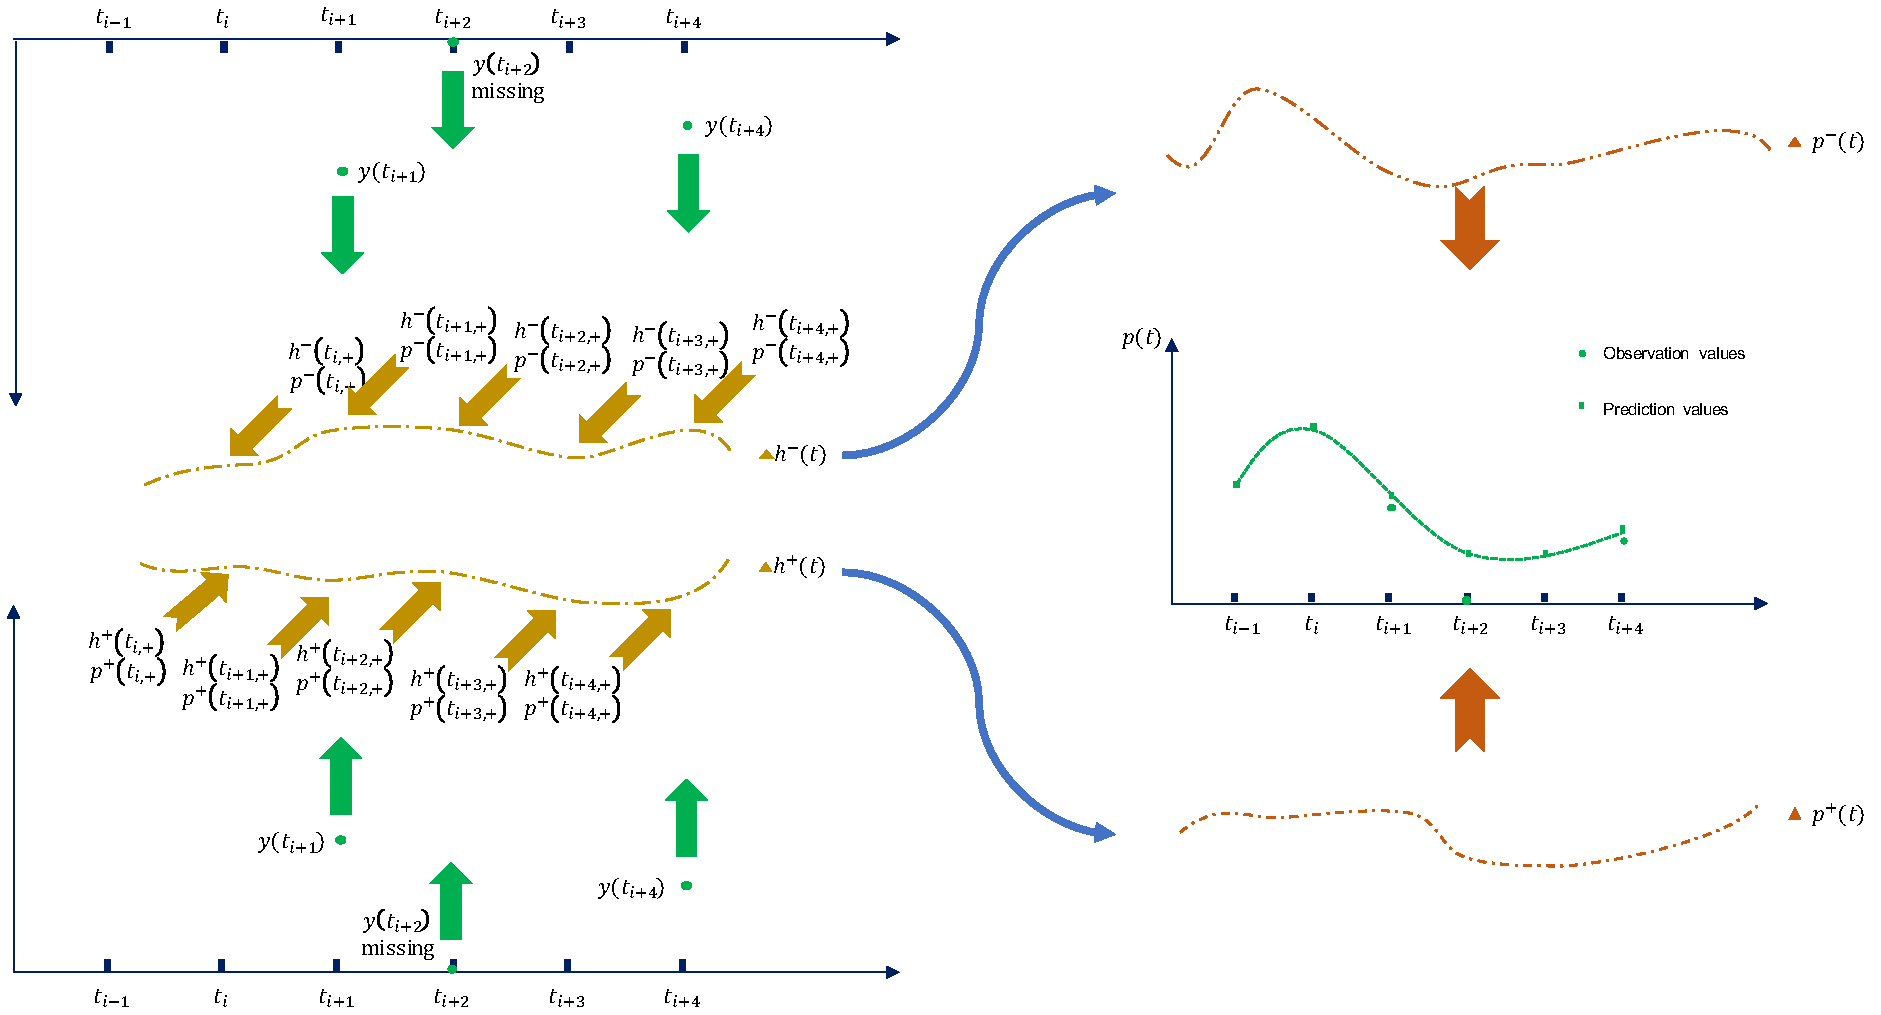
\includegraphics[width=0.9\textwidth]{picture/gruode_model.pdf}
    \caption{A concise diagram of deep learning model}
    \label{diagram}
    \end{figure}

There are two procedures to use deep learning method to interpolate the data.

\begin{enumerate}
    \item Feed all data into the model, and learn the time trend using the deep learning model.
    \item Use the tuned-parameter model to interpolate the data.
\end{enumerate}

And the interpolation results of deep learning model is shown in Fig. \ref{dl}.

\begin{figure}[h]
    \centering
    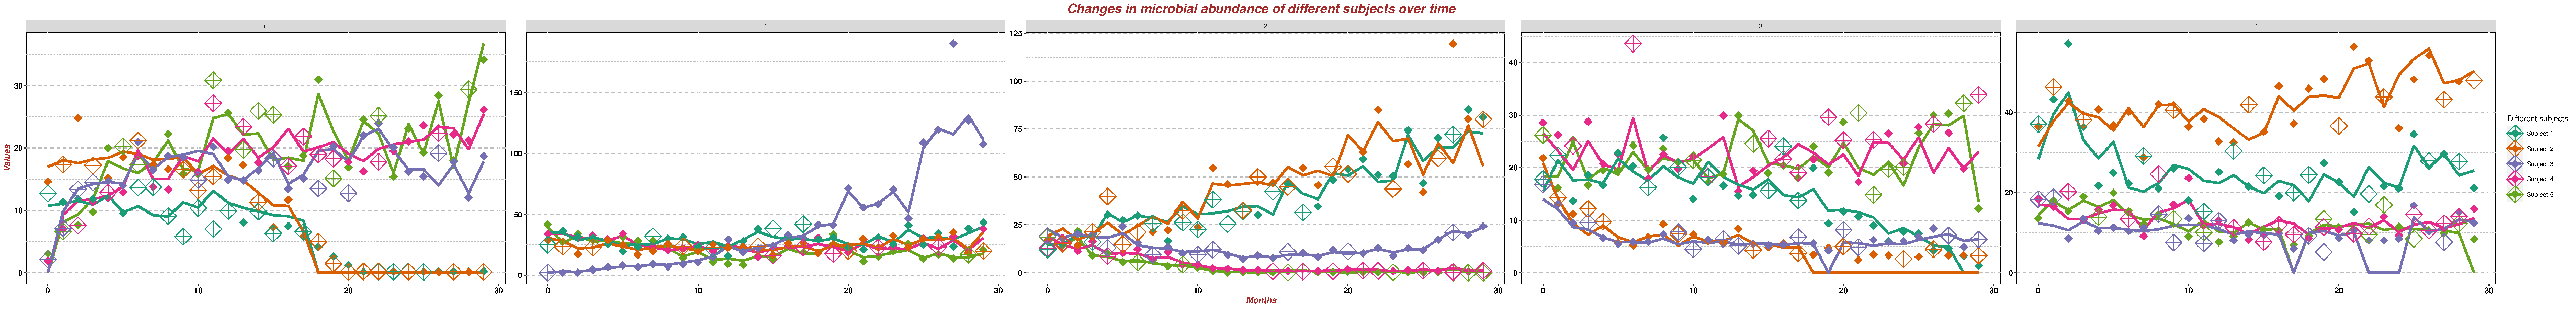
\includegraphics[width=0.9\textwidth]{figure/DL_spline.pdf}
    \caption{Results of deep learning interpolation}
    \label{dl}
\end{figure}

\subsection{B spline interpolation}

B-spline is widely used in nonparametric models in biomedical data. B-splines can be defined by construction by means of the Cox-de Boor recursion formula. Given a knot sequence $\ldots, t_{0}, t_{1}, t_{2}, \ldots$, then the Bsplines of order 1 are defined by
\begin{equation}
    B_{i, 1}(x):= \begin{cases}1 & \text { if } \quad t_{i} \leq x<t_{i+1} \\ 0 & \text { otherwise }\end{cases}
    \end{equation}
These satisfy $\sum_{i} B_{i, 1}(x)=1$ for all $x$ because for any $x$ exactly one of the $B_{i, 1}(x)=1$, and all the others are zero.
The higher order B-splines are defined by recursion
\begin{equation}
    B_{i, k+1}(x):=\omega_{i, k}(x) B_{i, k}(x)+\left[1-\omega_{i+1, k}(x)\right] B_{i+1, k}(x)
\end{equation}
where
\begin{equation}
\omega_{i, k}(x):= \begin{cases}\frac{x-t_{i}}{t_{i+k}-t_{i}}, & t_{i+k} \neq t_{i} \\ 0, & \text { otherwise }\end{cases}
\end{equation}

And the interpolation results of B-spline model is shown in Fig. \ref{bs}.

\begin{figure}[h]
    \centering
    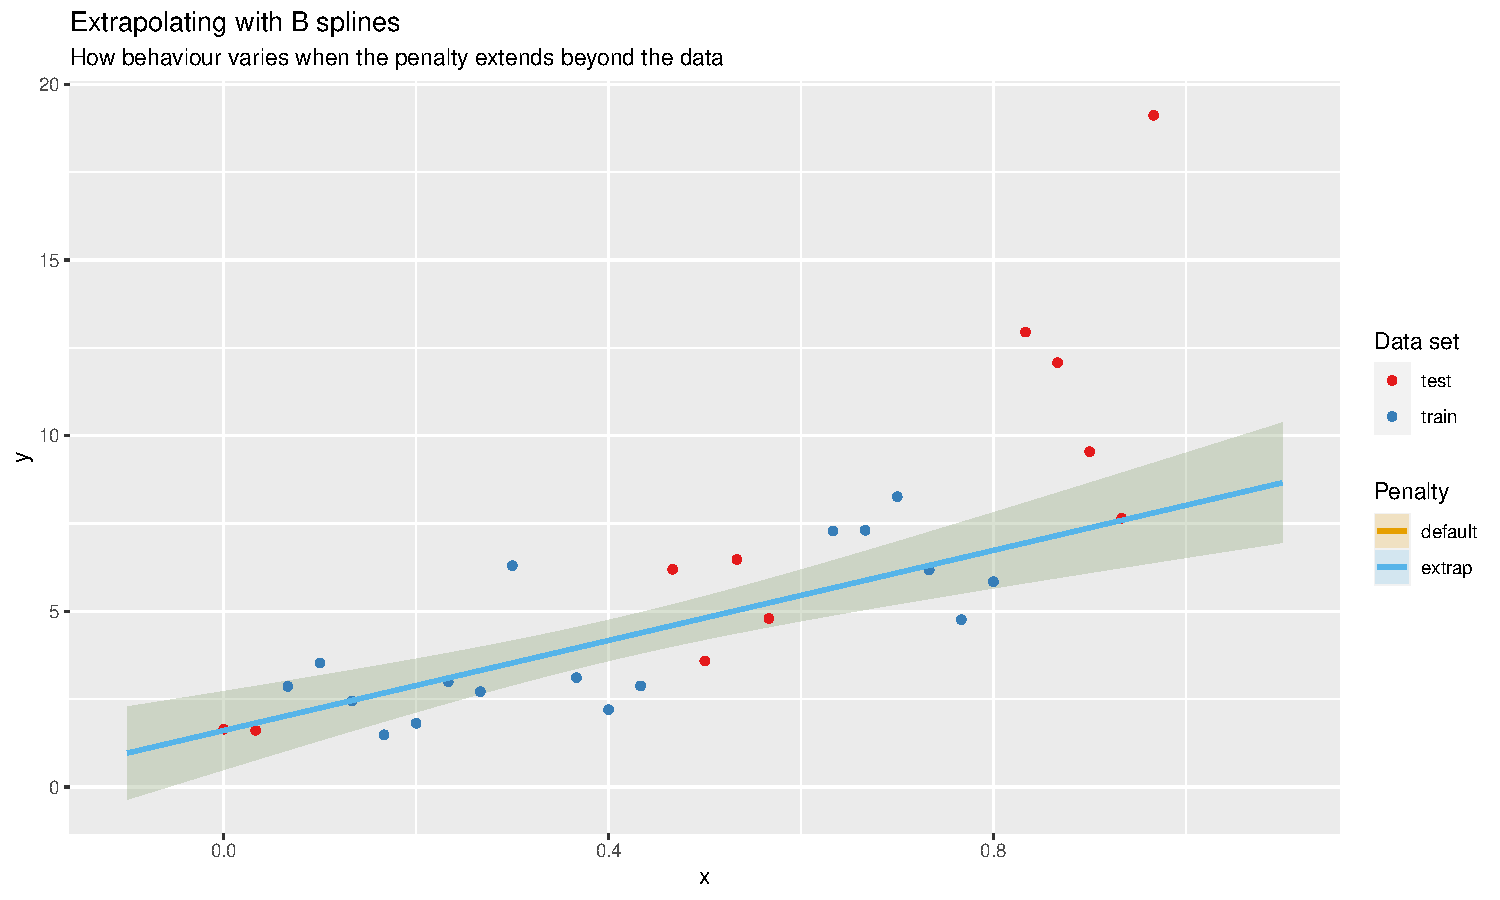
\includegraphics[width=0.9\textwidth]{figure/B_spline.pdf}
    \caption{Results of B spline interpolation}\label{bs}
\end{figure}


\subsection{Comparsion of the different interpolation methods}

We use MSE to compare the interpolation results of different methods.


\end{document}
